\apendice{Plan de Proyecto Software}

\section{Introducción}
El Plan de Proyecto Software es el documento clave que dirige el proceso de desarrollo de la aplicación móvil creada. Este apéndice tiene como objetivo detallar los aspectos críticos de la planificación y gestión del proyecto, asegurando una implementación eficiente y efectiva.
La planificación temporal del proyecto se ha llevado a cabo con el \emph{uso de la metodología ágil} buscando dividir el desarrollo en tareas, sprints e hitos que producen un resultado iterativos y bien estructurado, lo que conlleva a una mayor flexibilidad y a la adaptación más efectiva frente los cambios. 

A continuación, se determinará la viabilidad, que reflejará los \emph{recursos humanos y materiales}, así como los costes asociados necesarios para su valoración. La viabilidad incluirá una estimación de los fondos que se basarán en el salario de un trabajador simulado, así como un análisis de los posibles riesgos y su mitigación. Los aspectos económicos y técnicos de la viabilidad son fundamentales, ya que de ellos depende de que el proyecto esté en los límites establecidos y cumpla con los objetivos propuestos.

Este plan es esencial para la gestión del proyecto ya que sirve como una guía detallada, ayudando así a identificar y mitigar riesgos así como a la utilización eficaz de los recursos. Con el enfoque estructurado y ágil, proporcionado por este plan, el equipo de desarrollo podría entregar un producto de alta calidad que, además, cumplirá con el nivel de satisfacción alcanzado entre los usuarios o clientes. 
\section{Planificación temporal}
 Como se ha mencionado anteriormente, la planificación temporal del proyecto se ha llevado a cabo con el uso de metodología ágil: se basa en la división del desarrollo en tareas, sprints e hitos que producen un resultado iterativo y bien estructurado. Esto conlleva una mayor flexibilidad y a la adaptación más efectiva frente a los cambios.

 Algunas herramientas utilizadas para la planificación temporal han sido GitHub y Zube. Ésta última ha permitido la organización de las tareas en tableros Kanban o el uso de \textbf{métricas ágiles} con gráficos que sirven para evaluar el desarrollo del proyecto. Algunos de los artefactos más relevantes usados son los siguientes:
 \begin{itemize}
 	\item{\textbf{Gráficos burnup / burndown:}} muestran a lo largo del tiempo de un sprint la evolución de tareas realizadas por el equipo de desarrollo. En la explicación de los sprints se pueden ver los gráficos asociados al mismo
 \imagen{burnup-s6}{Gráfico Burnup del Sprint 6}{1}
 \item{\textbf{Gráfico de velocidad: }} permite comprobar el trabajo realizado en los diferentes sprints de manera que resulte lo más constante posible.
 \imagen{velocity}{Gráfico de velocidad de los sprints 1-10}
\end{itemize}
 A continuación veremos como la planificación temporal se ha llevado a cabo en diferentes sprints, cómo se ha ido iterando en las diferentes partes del proyecto y cómo se han ido cumpliendo los hitos propuestos. Para ello se mostrarán diferentes diagramas basadas en métricas ágiles.

 Cada tarea se ha dividido en diferentes historias de usuario, que se han ido completando en cada sprint. Cada sprint ha tenido una duración media de dos semanas, y se han ido completando las tareas propuestas en cada uno de ellos.
 Un ejemplo se puede observar en la siguiente figura ~\ref{fig:issue12}
 \imagen{issue12}{Tarea 12 mostrada en GitHub con la descripción, hito y etiquetas de la tarea a realizar.}

Gracias también al uso de \textit{Zube}, se ha podido llevar un control de las tareas a realizar, las tareas completadas y las tareas pendientes. Además, se ha podido llevar un control de los hitos propuestos y de las historias de usuario completadas en cada sprint. Un ejemplo de ello se puede observar en la siguiente figura ~\ref{fig:sprint1}
\imagen{sprint1}{Tablero Kanban de Zube con la gestión de tareas del Sprint 1.}

\subsection{\textit{Hitos}}
Los \textit{hitos o milestones} son puntos de referencia que marcan el final de un conjunto de tareas. En este proyecto se han definido los siguientes hitos:

\begin{itemize}

    \item \textbf{Kick-off} Completado el 30 de julio de 2024. Puesta en marcha del proyecto. A partir de las reuniones mantenidas con el tutor, se necesita tener todas las herramientas preparadas para empezar a desarrollar tanto la aplicación como su documentación.
    
    \item \textbf{MPV - Mínimo Producto Viable} Completado el 2 de septiembre de 2024. Se define el MVP como una aplicación móvil que sobre un mapa OSM muestre la ubicación de usuario, obtenga unos \acrshort{pdi} básicos y una ruta que las una.

    \item \textbf{Checkpoint 1 de documentación} Completado el 2 de septiembre de 2024. Este milestone agrupa las tareas relacionadas con la creación y actualización de la documentación del proyecto hasta la reunión con el tutor el 1 de septiembre de 2024.

    El objetivo es tener una documentación suficiente para que el tutor pueda dar feedback acerca de la misma y poder corregir errores.

    \item \textbf{Prototipo con tours generados por LLM} Completado el 1 de octubre de 2024. El objetivo es transitar desde una aplicación inicial capaz de mostrar lugares y rutas en un mapa, hacia una aplicación que sea capaz de conseguir que estos mismos marcadores y polilíneas sean generados a través de un LLM. \label{hito:prototipo_llm}
    
    \item \textbf{Prototipo Prompting} Completado el 15 de octubre de 2024. Este prototipo se puede realizar en un cuaderno Jupyter y su objetivo es mostrar la evolución en el prompt que dará como resultado unos \acrshort{pdi} de mayor calidad.
    
    \item \textbf{Desarrollo de aplicación completo} Completado el 12 de noviembre de 2024. Se consideran todas las funcionalidades que debe tener la aplicación a presentar como completadas.
    
    \item \textbf{Finalización \acrshort{tfg}:} Completado el 16 de enero de 2025. Se deja el proyecto en estado de entrega, completamente finalizado.
    
\end{itemize}

\subsection{Organización en \textit{Sprints}}

Al comenzar este proyecto durante periodo no lectivo se realizaron los Sprint con variación de tiempo de una o dos semanas en función de la planificación personal. Una vez comenzado el curso y con la ayuda del tutor se realizaron reuniones que han servido para, siguiendo la metodología \textit{Agile}, revisar el Sprint anterior, planificar el siguiente y hacer una pequeña retrospectiva para mejorar el trabajo conjunto.


\subsubsection{Sprint 0 - Kick-off(22/07/2024 - 29/07/2024)}
Después de las reuniones con el tutor, se establecen los objetivos del proyecto y se comienza a trabajar en la puesta en marcha del proyecto. Se establecen las herramientas a utilizar y se comienza a trabajar en la documentación del proyecto. 33 puntos de historia en 5 tareas:
    \begin{enumerate}
    	\item \textbf{Organización de repositorio.}
    	\item \textbf{Configuración de herramientas y equipos.}
    	\item \textbf{Trabajo en memoria I.}
    	\item \textbf{Investigación previa sobre LLM.}
    	\item \textbf{Determinación de ODS implicados.}
    \end{enumerate}
    
    
    \imagen{bd-kick-off sprint}{Figura burndown del Sprint Kick-off.}

\subsubsection{Sprint 1 - Investigación LLM y desarrollo básico de aplicación con mapa (29/07/2024 - 05/08/2024)} 
Con las herramientas y una idea previa establecida, es el momento de empezar a desarrollar.
    
    Objetivos: seguir formándome en LLM y las opciones que pueda implementar en el prototipo de prompt.
    Empezar a desarrollar la aplicación móvil con las características básicas.
    Aprender a documentar sprints, indicar qué elementos tendré que documentar y aquellos que tenga claro ir documentando para hacer un avance significativo que pueda evaluar mi tutor. 35 puntos de historia en 8 tareas:
    
    \begin{enumerate}
    	\item \textbf{Creación y organización proyecto base.}
    	\item \textbf{Bloc permiso GPS.}
    	\item \textbf{Bloc ubicación.}
    	\item \textbf{Mapa base OSM.}
    	\item \textbf{Intro, resumen y palabras clave.}
    	\item \textbf{Prompt sencillo en cuaderno Jupyter.}
    	\item \textbf{Probar modelo de ejemplo LangChain.dart.}
    	\item \textbf{Documentación del Kick-off sprint.}
    \end{enumerate}
        
    \imagen{bd-s1}{Figura burndown del Sprint 1.}
    
\subsubsection{Sprint 2 - Implementación solución GIS (05/08/2024 - 12/08/2024):} 
A partir del concepto básico, se añaden pequeñas mejoras en los tres aspectos del proyecto.
    
    Objetivos: mejorar el prototipo de prompting del cuaderno Jupyter hasta incorporar un sistema RAG, incluir marcadores al mapa en cuanto al desarrollo y continuar con la documentación. 26 puntos de historia en 6 tareas:

	\begin{enumerate}
		\item \textbf{Redacción de los objetivos del proyecto.}
		\item \textbf{Representación de marcadores en mapa.}
		\item \textbf{Inicio de Trabajos relacionados.}
		\item \textbf{Mostrar ubicación de usuario en el mapa.}
		\item \textbf{Wikivoyage como agente para RAG.}
		\item \textbf{Ingeniería del Prompting (cont.).}
	\end{enumerate}
        
    \imagen{bd-s2}{Figura burndown del Sprint 2.}
    
    \textit{Dificultades encontradas}: la documentación me hizo perder mucho tiempo debido a problemas con las librerías, después de mucho tiempo reinicié el proyecto desde la plantilla dada, insertando el texto, lo que solucionó el problema. En cuanto al diseño de la aplicación, el desarrollo fue lento al tener que evaluar diferentes opciones ya que la mayoría de fuentes utilizan mapas de Google, opción que se quería descartar.
 

\subsubsection{Sprint 3 - MPV(12/08/2024 - 22/08/2024):} 
Este sprint fue más largo que los anteriores para mejorar el resultado final ya que la intención era dejar el proyecto en un estado de revisión lo más completo posible para afrontar la reunión prevista para inicio de septiembre con el tutor del mismo. Al intentar desarrollar la tecnología de enrutado del usuario se comprendió lo que ya se intuía en el sprint anterior y es que basar el trabajo en servicios de Google iba a reportar en un desarrollo más fácil y un resultado más robusto y fiable como se justifica en la sección 5 de la memoria de este \acrshort{tfg}. 42 puntos de historia en 5 tareas:
    \begin{enumerate}
		\item \textbf{Obtención de marcadores POI.}
		\item \textbf{Crear ruta entre dos puntos.}
		\item \textbf{Trabajo inicial - Conceptos teóricos.}
		\item \textbf{Agent RAG.}
		\item \textbf{Adaptación a servicios Google.}
	\end{enumerate}
	\imagen{bd-s3}{Figura burndown del Sprint 3.}
    
    
\subsubsection{Sprint 4 - Servicios MapBox y LLM, preparación reunión inicio curso.(22/08/2024 - 02/09/2024)}
    El objetivo es mostrar la versión más completa de la aplicación, la documentación y ahondar en el uso de nuevas herramientas como Figma, una herramienta de diseño de aplicaciones y LangFlow a la hora de utilizar otro modelo de prototipo. 31 puntos de historia en 5 tareas:
\begin{enumerate}
	\item \textbf{Diseño de interfaz con Figma.}
	\item \textbf{Uso de Mapbox como geocoding.}
	\item \textbf{Marcadores POI y finalización MPV.}
	\item \textbf{Documentación para Checkpoint 1.}
	\item \textbf{LangFlow para Agent RAG.}
\end{enumerate}
    \imagen{bd-s4}{Figura burndown del Sprint 4.}
    
\subsubsection{Sprint 5 - Aplicación con origen de datos LLM (Preparación y documentación) (04/09/2024 - 14/09/2024)} 
Después de la reunión con el tutor de inicio de septiembre y habiendo cumplido los objetivos de los primeros hitos se decide continuar intentando alcanzar el hito \ref{hito:prototipo_llm}. Para ello se prepara y documenta primero en este sprint el desarrollo necesario. 28 puntos de historia en 6 tareas:
\begin{enumerate}
	\item \textbf{Revisión documentación memoria - resumen.}
	\item \textbf{Conceptos teóricos. Memoria.}
	\item \textbf{Técnicas y Herramientas. Mem. C.4.}
	\item \textbf{Modelo LLM en local.}
	\item \textbf{Route Optimization dependientes del medio.}
	\item \textbf{Generar icono y nombre de aplicación.}
\end{enumerate}
\imagen{bd-s5}{Figura burndown del Sprint 5.}

\subsubsection{Sprint 6 - Desarrollo y Finalización prototipo google\_generative\_ai como LLM (18/09/2024-01/10/2024)}
Habiendo encontrado una solución óptima al modelo LLM a utilizar se propone realizar un prototipo que implemente la interfaz de usuario y su conexión con el modelo LLM. En este sprint de gran avance en el desarrollo de la aplicación se consiguió reestructurar todo el código centralizando labores de gestión del tour generado y sus \acrshort{pdi} manteniendo la modularidad del código. 43 puntos de historia en 6 tareas:
\begin{enumerate}
	\item \textbf{Añadir tema a la aplicación.}
	\item \textbf{Loading screen.}
	\item \textbf{Modificar InfoWindow por Bottom Sheet.}
	\item \textbf{Marcador básico de POI a marcador con imágenes.}
	\item \textbf{Revisión documentación memoria v0.2.}
	\item \textbf{Rehacer 3.3 Conceptos acerca de los modelos.}
	\item \textbf{Estudiar guardado de rutas.}
	\item \textbf{Reorganización de proyecto: Clase Eco City.}
\end{enumerate}
\imagen{bd-s6}{Figura burndown del Sprint 6.}
	
\subsubsection{S7 - Consolidación y Calidad (02/10/2024 - 22/10/2024)} Habiendo cumplido el hito \ref{hito:prototipo_llm} y teniendo una aplicación con muchas funcionalidades implementadas, durante este sprint se busca consolidar el código y dotarlo de una calidad y mantenimiento con herramientas de soporte como Sonar Cloud o Logger. 39 puntos de historia en 9 tareas:
\begin{enumerate}
	\item \textbf{Establecer Requisitos.}
	\item \textbf{Límite a la extensión del Eco City Tour.}
	\item \textbf{Tour Screen: pantalla de resumen del tour.}
	\item \textbf{Diagramas de paquetes/componentes.}
	\item \textbf{Finalización prototipo Langflow.}
	\item \textbf{Finalización prototipo Jupyter Notebook.}
	\item \textbf{Instalación de Logger.}
	\item \textbf{Integración de Sonar Cloud.}
	\item \textbf{Convocatoria Prototipos Orientados al Mercado.}
\end{enumerate}
\imagen{bd-s7}{Figura burndown del Sprint 7.}

\subsubsection{S8 - Cobertura de tests y guardado de rutas (23/10/2024 - 12/11/2024)}
Se procede a implementar las últimas funcionalidades del desarrollo de la aplicación. Además, se busca que la integración con sonarcloud confirme que se trabaja con un standard de calidad para lo que se necesita la cobertura de tests y por último se retoma el trabajo de documentación. 29 puntos de historia en 7 tareas:
\begin{enumerate}
	\item \textbf{Configurar tarea de despliegue continuo Flutter.}
	\item \textbf{Guardar Eco City Tour.}
	\item \textbf{Corrección de diagramas.}
	\item \textbf{Revisión de memoria/anexos.}
	\item \textbf{Guardado de log compartido.}
	\item \textbf{Investigación de opciones Google para base de datos.}
	\item \textbf{Tests de aplicación / Cobertura.}
\end{enumerate}
\imagen{bd-s8}{Figura burndown del Sprint 8.}

\subsubsection{S9 - Testing y selección de perfil de asistente \acrshort{ia} (13/11/2024 - 03/12/2024)}
En este sprint se exploró la posibilidad de generar diferentes perfiles de asistente, asignando al modelo roles específicos para personalizar las respuestas generadas. También se avanzó significativamente en la evaluación del código mediante la implementación de tests. Además, se inició la redacción de algunos apartados de los anexos relacionados con la documentación del proyecto. 56 puntos de historia distribuidos en 10 tareas:
\begin{enumerate}
	\item \textbf{Test: servicios, modelos, repositorios. Pruebas.}
	\item \textbf{Anexo E - Documentación de usuario.}
	\item \textbf{Anexo D - Documentación T. de programación.}
	\item \textbf{Anexo A3 - Estudio de viabilidad.}
	\item \textbf{Refinamiento final de prompting.}
	\item \textbf{Limpieza de repositorio.}
	\item \textbf{Test: gestor de estados Bloc.}
	\item \textbf{Añadir selección de asistente AI.}
	\item \textbf{Apéndice C.}
	\item \textbf{Revisión final memoria.}
\end{enumerate}
\imagen{bd-s9}{Figura burndown del Sprint 9.}

\subsubsection{S10 - Wiki, internacionalización, anexos, workflow ci (16/12/2024 - 20/12/2024)}
Se estudia la posibilidad de generar diferentes asistentes dándole al modelo distintos roles. Se pretende realizar el test que llevará la aplicación en este sprint. Además, tendrá se realizará el inicio de apartados de anexos en cuanto a documentación. 56 puntos de historia en 10 tareas:
\begin{enumerate}
	\item \textbf{Wiki.}
	\item \textbf{Internacionalización.}
	\item \textbf{Documentación de la programación (código).}
	\item \textbf{Limpieza de repositorio.}
	\item \textbf{Workflow Integración Continua.}
	\item \textbf{Integración continua a manual de programador.}
	\item \textbf{Mejoras en anexos.}
	\item \textbf{Anexo de Diseño.}
\end{enumerate}
\imagen{bd-s10}{Figura burndown del Sprint 10.}

\subsubsection{S11 - Finalización \acrshort{tfg} (23/12/2024 - 09/01/2025)}
Último sprint dedicado a finalizar las últimas funcionalidades, terminar la documentación y realizar los vídeos, en definitiva todos los elementos preparados para la entrega del \acrfull{tfg}. 39 puntos de historia en 7 tareas:
\begin{enumerate}
	\item \textbf{Revisión Anexo: planificación y análisis.}
	\item \textbf{Internacionalización 2.}
	\item \textbf{Mejora del README.md: Añadir insignias de herramientas utilizadas.}
	\item \textbf{Video de presentación.}
	\item \textbf{Video de demostración.}
	\item \textbf{Revisión anexo de diseño y manual de usuario.}
	\item \textbf{Adaptación de Memoria a la longitud permitida.}
\end{enumerate}
\imagen{bd-s10}{Figura burndown del Sprint 11.}
\todo{CAMBIAR EL DIAGRAMA!}



\section{Estudio de viabilidad}
En esta sección se analizan los aspectos clave para determinar si la implementación del proyecto y el desarrollo de la aplicación móvil \textit{Eco City Tours} es viable desde un punto de vista legal y económico. Se destacan los valores positivos de la aplicación, como su independencia de intereses particulares y su enfoque sostenible, que la convierten en una propuesta valiosa en el mercado del fomento del turismo sostenible. Se evaluará si los beneficios esperados compensan los costes de desarrollo, el mantenimiento de los servicios y los posibles problemas legales, determinando así su viabilidad.
\subsection{Viabilidad económica}
\subsubsection{Costes de personal}
El desarrollo de la aplicación se realiza con un grupo de trabajo de un solo empleado de categoría profesional equivalente a la de un Ingeniero Informático. Según el XVIII Convenio Colectivo Estatal de Empresas de Consultoría, Tecnologías de la Información y Estudios de Mercado y de la Opinión Pública, publicado en el BOE el 26 de julio de 2023 \cite{boe2023_consultoria} podría estar entorno a los 2.000 € antes de impuestos.

\tablaSmallSinColores
{Costes de \textit{personal}} % Título de la tabla
{lc} % Formato de las columnas (l: izquierda, c: centrado)
{costes-personal} % Etiqueta para referencias cruzadas
{%
	\textbf{Concepto} & \textbf{Coste} \\ % Cabecera
}
{%
	Salario Desarrollador & 1.500€  \\ 
	Retenciones y Seguridad Social & 500 \\
	\midrule
	\textbf{Total 4 meses} & \textbf{8.000€} \\ 
}

\subsubsection{Coste de hardware}
Para calcular el coste de los equipos se supone un período de amortización de 3 años para todo el hardware. Para realizar Eco City Tours se usará un ordenador de sobremesa con procesador i7 y 16 Gb de memoria RAM capaz de utilizar los programas necesarios para el desarrollo de manera fluida. Se tienen en cuenta también periféricos para dicho equipo y un teléfono móvil Android para pruebas de implementación en un dispositivo real no virtualizado. Por tanto y a modo resumen tenemos:

\tablaSmallSinColores
{Costes de \textit{hardware}} % Título de la tabla
{lcc} % Formato de las columnas (l: izquierda, c: centrado)
{costes-hardware} % Etiqueta para referencias cruzadas
{%
	\textbf{Concepto} & \textbf{Coste} & \textbf{Coste amortizado} \\ % Cabecera
}
{%
	Ordenador & 1.200€ & 400€ \\ 
	Periféricos & 240€ & 80€ \\ 
	Teléfono móvil Android & 300 & 100 \\
	\midrule
	\textbf{Total} & \textbf{1.740€} & \textbf{580€} \\ 
}

Asociado a estos costes también podremos asociar el \textbf{uso de Internet} necesario para poder desarrollar sin problemas buscando información o descargando paquetes necesarios del repositorio de Flutter. Un servicio básico de este tipo \textbf{puede costar 30-60 euros} dependiendo de la velocidad del mismo o de otros productos asociados al cliente.
	
\subsubsection{Coste de software}
El software utilizado para el proyecto es libre. Visual Studio Code como IDE de desarrollo único, libre y gratuito y Android Studio en su versión gratuita para poder instalar emuladores de dispositivos móviles. El paquete SDK de Flutter no supone tampoco ningún gasto por parte del desarrollador.
Como sistema operativo se sugiere Ubuntu 22.04 LTS ya que tiene soporte a largo plazo, se trata de un entorno estable, confiable y se trata de una versión de código abierto. La herramienta y extensión de Visual Studio Code Copilot aunque útil no es imprescindible pudiendo usar . El resto de software para prototipado como Langflow o LMStudio son también gratuitos.

\subsubsection{Coste de los Servicios Google}
Durante el desarrollo de la aplicación la empresa incurrirá en gastos por uso de estos servicios. Una forma de pago tiene que estar asociada al proyecto y sobre el mismo se podrán asociar todas las API y servicios asociados al mismo: Firebase, Google Directions, Google Maps, Generative AI tienen gastos asociados. Sin embargo, el desarrollador tendrá un período de prueba de 3 meses donde no se cargará ningún gasto siempre que no supere los 300 euros. 
\begin{figure}[h!]
	\centering
	\includegraphics[width=0.8\textwidth]{trafico\_google} % Ruta del archivo de la imagen
	\caption{Tráfico de peticiones durante el desarrollo de \textit{Eco City Tours}} % Pie de la imagen
	\label{fig:trafico_google} % Etiqueta para referenciar
\end{figure}

Desde la experiencia durante el desarrollo las peticiones están lejos de incurrir en gastos. En el período de pruebas donde se realizaron las mayores peticiones a los servicios como se puede ver en la imagen \ref{fig:trafico_google} el coste llegó a los 40 euros, muy lejos de los 300 que supondrían un gasto para el desarrollador.

\begin{figure}[h!]
	\centering
	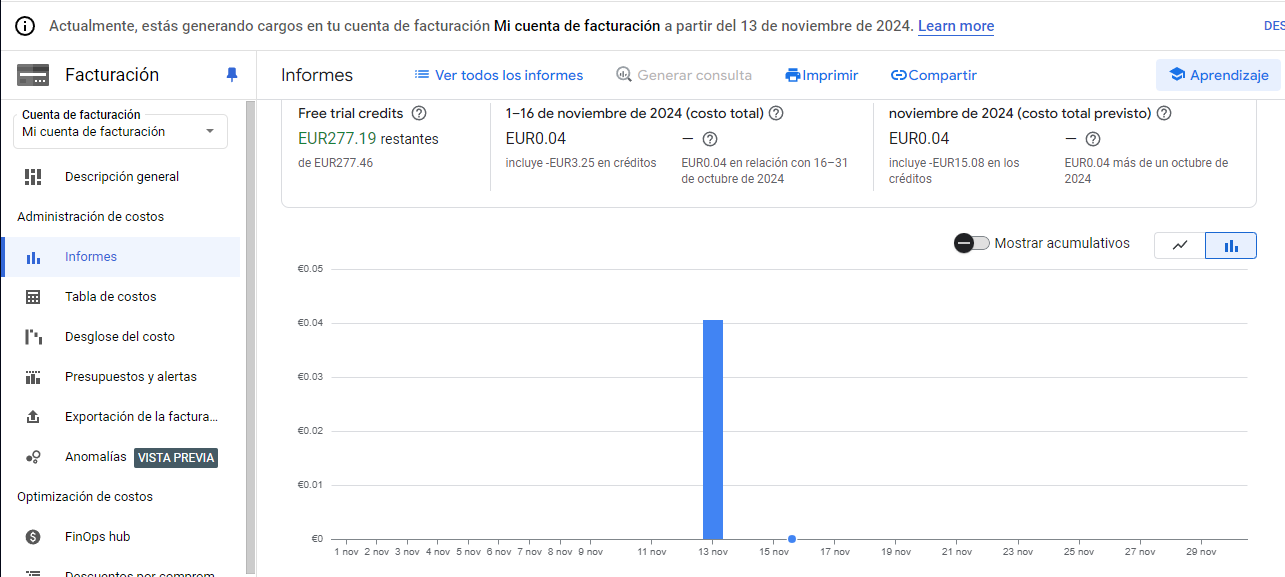
\includegraphics[width=0.8\textwidth]{cloud-console} % Ruta del archivo de la imagen
	\caption{Interfaz de Facturación de Cloud Console.} % Pie de la imagen
	\label{fig:cloud_console} % Etiqueta para referenciar
\end{figure}

Pasado el período de tres meses, la cantidad que supone un umbral de coste se reduce a los 200 euros. En la imagen \ref{fig:cloud_console} se puede ver como se inicia otro proceso de facturación diferente. Supondría por tanto algo a tener en cuenta si se despliega la aplicación en versiones tempranas en el repositorio de aplicaciones de Android puesto que las peticiones no serían solo de una persona, en este caso el desarrollador sino del público en general. La misma consideración habría que hacer si durante el desarrollo se cede el proceso de pruebas a varias personas que puedan hacer la función de beta-testers disparando el consumo de peticiones y por tanto el gasto.
Para el caso de Eco City Tours se supone que el desarrollo y el mayor volumen de peticiones se concentran en los tres primeros meses donde el umbral de gasto es más alto, las pruebas las realiza el propio desarrollador que tendrá acceso al panel de Google Cloud para controlar los posibles gastos y la publicación de la aplicación será en un momento en el que el propio beneficio generado contrarreste los gastos en los que se pueda incurrir.
\subsubsection{Conclusiones}
\textbf{El desarrollo de la aplicación se estima en 4 meses} por el equipo auto gestionado por un solo desarrollador. No se tienen en cuenta alquileres de oficinas o co-working ya que se plantea la posibilidad de teletrabajar, pudiendo trabajar de manera deslocalizada ahorrando así costes. Teniendo en cuenta lo anteriormente citado obtenemos la siguiente tabla resumen:
\tablaSmallSinColores
{Costes totales de \textit{Eco City Tours}} % Título de la tabla
{lc} % Formato de las columnas (l: izquierda, c: centrado)
{costes-totales} % Etiqueta para referencias cruzadas
{%
	\textbf{Concepto} & \textbf{Coste}  \\ % Cabecera
}
{%
	Mano de obra & 8.000€ \\ 
	Hardware & 580€  \\ 
	Internet & 135€ \\ 
	Software & 0€ \\ 
	Servicios Google & 0€ \\ 
	Revisión y auditoría del tutor & 750€ \\ 
	\midrule
	\textbf{Total} & \textbf{9.465 €} \\ 
}

Se ha incluido un coste estimado de 750 € por las tareas de \textbf{revisión y auditoría realizadas por el tutor}. Este coste considera una dedicación de 30 horas, remuneradas a un coste promedio de 25 €/hora, que incluye reuniones, revisiones parciales y finales del proyecto.


Una vez analizado los costes devengados de la creación de la aplicación el beneficio de su explotación debe ser mayor al gasto ocasionado por su creación. Además, una vez publicada la aplicación en la \textit{Play Store} el beneficio obtenido por su explotación debe compensar el tiempo requerido por el personal en horas de mantenimiento de los posibles problemas que pueda experimentar como por ejemplo problemas por actualización de los componentes claves como modelos LLM, que puedan quedar obsoletos. El beneficio de la aplicación puede provenir de varias fuentes en función del modelo de explotación que se eligiese:
\begin{itemize}
	\item \textbf{Ingresos por descarga:} si la aplicación tiene un precio por descarga, los ingresos corresponderían al dinero obtenido menos una comisión del 15\% cobrada por Google por cada venta \cite{googleplay_commission}. Inicialmente, se propone un precio aproximado de lanzamiento de 5 euros, considerando que se obtendrían aproximadamente 4,40 euros como beneficio por descarga. Este precio se estima razonable para incentivar descargas durante la fase inicial. Tras un periodo de prueba, el precio podría ajustarse en función del número de descargas y del comportamiento de los usuarios. Los gastos derivados del uso de servicios externos, como peticiones a APIs, se compensarían con un equilibrio entre usuarios que realicen menos consultas y aquellos más demandantes, garantizando siempre un beneficio estimado en el modelo económico.
	
	\item{Publicidad:} empresas o entidades colaboradoras podrían financiar el desarrollo con publicidad siempre que ésta no suponga una perdida de independencia en los resultados de los modelos, fomente el turismo ecológico y no sea invasiva ni perjudique la experiencia de usuario.
\end{itemize}

\subsection{Viabilidad legal}
Al utilizar los servicios ofrecidos por Google, la compañía se convierte en un socio en el que se delegan muchas de las responsabilidades legales, técnicas y de cumplimiento normativo. Esto simplifica la implementación de Eco City Tours, a la vez que se adquieren ciertos compromisos con el gigante tecnológico. 

\subsubsection{Licencias de uso de las API de Google}
Cada API tiene sus propios términos de uso \cite{google_cloud_terms} y se tiene que tener en cuenta los siguientes aspectos:
\begin{itemize}
	\item \textbf{Uso permitido:} Las API deben ser utilizadas únicamente para finalidades relacionadas con el proyecto.
	\item \textbf{Prohibiciones:} Se prohíbe el \textit{scraping}, almacenamiento de datos más allá de los límites permitidos o redistribución no autorizada.
\end{itemize}

Restricciones específicas:
\begin{itemize}
	\item \textit{Generative AI:} Regulada por políticas relacionadas con el uso de datos generados, especialmente en contextos comerciales.
	\item \textit{Places API y Directions API:} Restringen el almacenamiento y redistribución de los datos obtenidos.
	\item \textit{Maps SDK for Android:} Requiere incluir el logotipo de Google y atribuciones visibles en la interfaz.
\end{itemize}

Los servicios de Google tienen modelos de precios basados en uso para lo que es legalmente\textbf{ obligatorio registrar un método de pago válido} en tu cuenta de Google Cloud para garantizar la continuidad del servicio.

\subsubsection{Privacidad de datos}

El cumplimiento de normativas sobre protección de datos es fundamental:

\begin{itemize}
	\item \textbf{GDPR:} Si se cumplen algunos de los trabajos futuros de la aplicación, ésta recogería datos del usuario, si es un ciudadano europeo debe:
	\begin{itemize}
		\item Firmar un \textit{Acuerdo de Procesamiento de Datos} (DPA) con Google.
		\item La aplicación debe mostrar cómo se manejan los datos obtenidos.
	\end{itemize}
\end{itemize}

Se debe informar a los usuarios que los datos están sujetos a las Políticas de privacidad de Google.

\subsubsection{Restricciones geográficas}

Algunas API tienen restricciones en determinados países debido a leyes locales o sanciones internacionales. 


\subsubsection{Propiedad intelectual}

Los datos obtenidos a través de las API de Google (como mapas y lugares) son propiedad intelectual de Google.


\begin{itemize}
	\item \textbf{Prohibiciones:}
	\begin{itemize}
		\item No se puede almacenar ni redistribuir datos más allá de los límites permitidos.
		\item No se puede usar los datos para minería o análisis masivo sin autorización.
	\end{itemize}
\end{itemize}

\subsubsection{Cumplimiento con normas de publicación}

Para poder publicar la aplicación en el repositorio de aplicaciones Android hay que especificar claramente la política de privacidad y detallar el uso de los servicios.


\subsubsection{Lista a cumplir para viabilidad legal}

\begin{enumerate}
	\item Revisar términos de uso de cada API.
	\item Registrar método de pago.
	\item Cumplir con las normativas de privacidad (GDPR, CCPA).
	\item Incluir atribuciones visibles en la interfaz de usuario.
	\item Respetar las restricciones de almacenamiento y uso de datos.
	\item Desarrollar y publicar una política de privacidad clara para los usuarios.
\end{enumerate}

Respetando el uso ético de la aplicación y cumpliendo con estos requisitos la viabilidad legal de Eco City Tours estaría cumplida y no supondría un impedimento para su ejecución.